\documentclass[]{scrartcl}
\usepackage[utf8]{inputenc}
\usepackage[spanish]{babel}
\usepackage{graphicx}
\usepackage{color}
\usepackage[usenames,dvipsnames,svgnames,table]{xcolor}
\usepackage{hyperref}
\usepackage{url}
\hypersetup{
	colorlinks   = true,
	citecolor    = gray,
	urlcolor     = darkgray,
	linkcolor	 = darkgray
}

%opening
\title{Sistemas Inteligentes para la Gestión en la Empresa\\-\\Práctica 2: Deep Learning para multi-clasificación}
\author{Carlos Cobos Suárez\\Adrián Morente Gabaldón}

\begin{document}

\maketitle
\newpage
\tableofcontents
\newpage

\section{Introducción}

En este proyecto vamos a realizar diversas aproximaciones al tratamiento de técnicas de \textbf{aprendizaje profundo} con el lenguaje \textbf{\textit{R}}. Tras ponernos en situación con los fundamentos teóricos necesarios para entender el desarrollo realizado, comentaremos las soluciones pensadas y las que finalmente se hayan implementado; realizando después una discusión de los resultados obtenidos.\\

El conjunto de datos (o \textit{dataset}) que utilizaremos se corresponde con el de \textbf{\textit{PetFinder.my Adoption Prediction}}, y podemos encontrarlo en la plataforma \href{https://kaggle.com}{Kaggle} \cite{petfinder-dataset}. Los datos contenidos clasifican un histórico de perros y gatos alojados en centros de adopción de animales, con diversas características y almacenando el \textbf{tiempo de adopción} de cada una de estas mascotas.\\

El trabajo a desarrollar en este proyecto versa sobre el \textbf{entrenamiento de modelos de predicción} que, a partir de imágenes o de un conjunto de características de animales, clasifiquen éstos por tiempo de adopción. Utilizaremos \textbf{cinco categorías} (las cuales se ordenan según el tiempo de adopción en orden ascendente).\\

Dado que para el entrenamiento se dispone de un gran conjunto de datos ya clasificado, realizaremos algún \textbf{histograma}, lo que trata de un gráfico de barras que muestra el cardinal del conjunto de datos de cada una de las distintas categorías mencionadas.

\section{Fundamentos teóricos}

	Para entender tanto la finalidad del proyecto como los pasos realizados para su compleción, debemos ubicarnos en un marco teórico apropiado. Para empezar, antes de abordar la temática relacionada con el \textbf{aprendizaje profundo}, debemos hablar del \textbf{aprendizaje automático} y las técnicas más destacadas para su puesta en uso, como pueden ser las \textbf{redes neuronales} de diversos tipos.
	
	\subsection{Redes neuronales}
	
		Sabemos que la unidad básica de una red neuronal es, lógicamente, la \textbf{neurona}; cuya función es recibir unos datos de entrada, procesarlos mediante algunas operaciones matemáticas, y producir una salida.\\
		
		Estas entradas pueden provenir de la entrada al sistema o de la salida por parte de otras neuronas. Además, el número de éstas es variable, como podemos ver en la figura \ref{neuron}, donde se visualiza un ejemplo de neurona con 2 entradas y 1 salida.
	
		\begin{figure}[h]
			\centering
			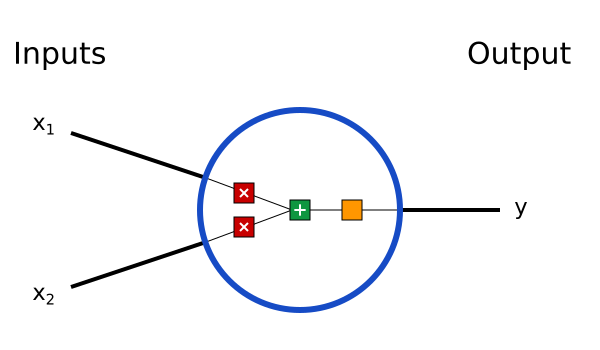
\includegraphics[width=0.5\textwidth]{./img/neuron}
			\caption{Neurona simple con dos entradas y una salida.}
			\label{neuron}
		\end{figure}
	
	\subsection{Redes neuronales convolucionales}
	
	\subsection{\textit{Deep Learning}}
	
		Se conoce como \textbf{aprendizaje profundo} al campo de aplicación del \textbf{aprendizaje automático} donde se hace un uso más extenso de técnicas basadas en \textbf{redes neuronales artificiales}. Estas redes utilizadas son capaces de aprender \textit{profundamente} para trabajar con problemas como reconocimiento de imágenes, de texto o de voz; además de otras aplicaciones como filtrado colaborativo en redes sociales y visión por computador.\\
		
		La diferencia principal entre una red neuronal simple y las redes de \textit{aprendizaje profundo} reside en que las primeras contienen una suma de tres capas: la de \textbf{entrada}, la \textbf{intermedia} (donde se aplican las operaciones) y la de \textbf{salida}.\\
		
		Por otro lado, en las redes neuronales de \textit{deep learning} el número de capas intermedias es mayor, con lo que se consigue un mejor aprendizaje. Esto se debe a que el número de neuronas (y por tanto de pesos en el modelo final) es mayor; y cuanto más alto sea el número de hiperparámetros presentes en un algoritmo, mayor es la capacidad de entrenamiento que tendrá dicho modelo final.
		
		\begin{figure}[h]
			\centering
			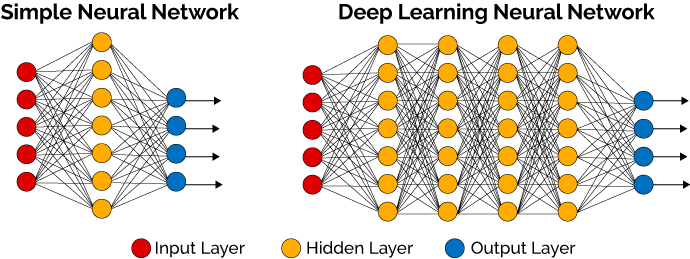
\includegraphics[width=0.8\textwidth]{./img/neural-network-differences}
			\caption{Diferencia entre red neuronal simple y red de aprendizaje profundo.}
			\label{nn-differences}
		\end{figure}
	
		\subsubsection{Modelos de clasificación}
		
		\subsubsection{Técnicas de binarización}
		
		\subsubsection{\textit{Ensembles}}

\section{Descripción de las redes empleadas}

	\subsection{Primera aproximación - Red vista en clase}
	
	\subsection{Segunda aproximación - Balanceo de clases}
	
	funciona con pesos. como tenemos los datos del histograma, podemos sacar los porcentajes (pesos) a utilizar para que estén balanceados con el resto de clases.
	
	\subsection{Tercera aproximación - \textit{Data augmentation}}
	
\section{Discusión de resultados}

\section{Conclusiones}

\bibliographystyle{plain}
\bibliography{sources}

\end{document}
